\setchapterpreamble[u]{\margintoc}
\chapter{Creativity and Decision Making with Deep Learning Models}
\labch{intro}

\textit{"AI Policy}

\textit{I expect you to use AI (ChatGPT and image generation tools, at a minimum), in this class. In fact, some assignments will require it. Learning to use AI is an emerging skill, and I provide tutorials in Canvas about how to use them. I am happy to meet and help with these tools during office hours or after class}

\textit{Beware of the limits of ChatGPT:}

\begin{itemize}
	\item\textit{If you provide minimum effort prompts, you will get low quality results. You will need to refine you prompts to get good outcomes. This will take work.}
	\item\textit{Don't trust anything it says. If it gives you a number or a fact, assume it is wrong unless you either know the answer or can check in with another source. You will be responsible for any errors or omissions provided by the tool. It works best for topics you understand.}
	\item\textit{AI is a tool, but one that you need to acknowledge using. Please include a paragraph at the end of any assignment that uses AI explaining what you used the AI for and what prompts you used to get the results. Failure to do so is in violation of academic honesty policies}
	\item\textit{Be thoughtful about when this tool is useful. Don't use it if it isn't appropriate for the case or circumstance."}
\end{itemize}

\textit{Dr. Ethan Mollick, 2023 - Syllabus for class at The Wharton School at the University of Pennsylvania}


\section{Theories of Creativity}

Machine learning models use data (from the past) to discover rules and make classifications. Because of the way they are constructed these classifications, suggestions, artworks are by definition derivative or "having parts that originate from another source". I won't get into a philosophical discussion on what the nature of creativity is, but it's worth considering how using deep learning AI models biases us towards the past, but also could give us insights from other domains. 

\begin{marginfigure}[-5.5cm]
        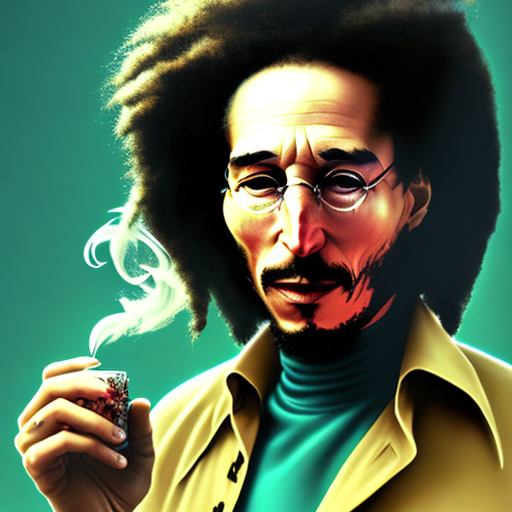
\includegraphics{jobsweed}
        \caption{"mdjrny-v4 Steve Jobs Smoking weed with Bob Marley 8k" made with Mann-E. It's 100\% derivative, but it's art too (I guess).}
        \labfig{jobsweed}
\end{marginfigure}

It can be argued that creativity is simply the combination of existing works. This is because many new ideas and innovations are often inspired by and built upon existing concepts. For example, a new form of music may be created by combining elements from different genres. Similarly, a new technology may be created by combining and improving upon existing technologies.

It can also be argued that creativity involves much more than just combining existing works. Creativity is not just about recombining existing ideas, but also about coming up with completely new and original concepts. This requires a unique perspective and a deep understanding of the subject matter, as well as the ability to think outside the box.  

AI models of speech, when heavily used, may slow down the evolution of language. AI art models may slow down "progress" in art, whatever that means. AI models of disease trained on data from 1980 may be irrelevant to today's diseases\sidenote{We'll discuss "concept drift" later, don't worry.}. That said these same models may give us interesting insights in new domains, models trained on beautiful paintings may be put to use in a new domain (like desiging beautiful interiors) and that model could give new insight to interior designers, models of the interaction of ants could be put to use in designing cities and so on and so forth. AI cuts many ways, it makes us faster but makes us more reliant on the past, models can be used across domains but should be used intentionally and transparently when possible. Each use opens up a new world of possibilites for users, and sometimes a new headache for intellectual property lawyers. We'll discuss all of these topics in this chapter.


\section{Creative Uses of Power Tools}

Power tools, even simple ones like a drill\sidenote{something like these \url{https://www.dewalt.com/products/power-tools/drills}} are complex machines that take human input and transform it using static rules. The pressure the user of a drill puts on the bit and the speed at which they pull the trigger all deterministically affect the output. Just because a tool is a deterministic machine doesn't mean it is unable to produce creatve works.

What is happening as we use generative tools like ChatGPT or image-to-textmodels is that the "creative act" has been relocated. The creative act is now the prompt you give the tool, the users input. And someone can still be good at using AI, just like someone can be good at using any piece of software.

Modern AI is a complex system of algorithms, data, and analytics that can be used to solve complex problems. AI systems can learn from data, identify patterns, and make predictions about the future. AI systems are typically used to automate and assist human decision making. AI systems are programmed with specific objectives and goals, and the user input decides the output. For example, an AI system could be programmed to solve a mathematical problem and the user input would determine the parameters of the problem and the output would be the solution.

A power drill is also a complex deterministic system. The user input is limited to the type of drill bit, the speed of the drill, and the direction of the drill. The output is determined by these inputs, as the drill will only drill in the direction and speed determined by the user. The user also has to choose the correct drill bit to ensure the drill can do the job correctly and safely.

\begin{marginfigure}[-5.5cm]
        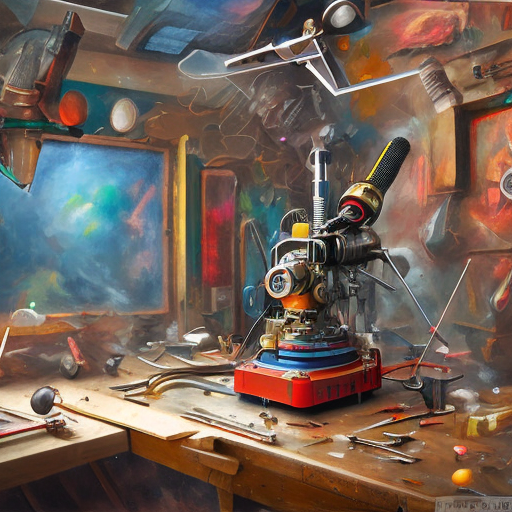
\includegraphics{drillart}
        \caption{"mdjrny-v4 a mikita drill being used in an artist's studio to make a colorful artwork 8k" made with Mann-E}
        \labfig{drillart}
\end{marginfigure}

Overall, both modern AI and a power drill are complex but ultimately deterministic systems. The user input, however limited it may be, ultimately controls the output of the system. Both systems require a user to understand how to use them and to make the correct input to get the desired output.

\section{Garbage In, Garbage Out}

The "Power Tool" of AI is a deterministic \sidenote{and static or unchanging} system and the rules of that system are determined by the data that the model is shown. If a model is trained on shitty\sidenote{scientific term here} data, it will produce shitty results. End of book...

... maybe not. It's worth thinking about this for a moment. It is often said that modern AI can "generalize and make informed inferences given new data". If deep learning models are really just a big regression, these models will always come up with an answer, but if the world changes, these models will still be projecting complicated averages of their past data into the future.\sidenote{I'm going to talk about concept drift in a few paragraphs, I promise} 

So, let's separate AI's decision making into two extremes; \textit{Creative Decision Making} and \textit{Critical Decision Making}. The stakes are very low in a world of \textit{Creative Decision Making} and who gives a shit if the AI is all a regression, and it just mushes together the limited data that it's seen. In a creative context you can also ask an AI interesting questions, so long as you don't soley rely on it's output without checking the facts first\sidenote{see the syllabus note at the beginning of this chapter}. Even if "Garbage In, Garbage Out" holds, garbage can still be helpful for a creative process. 

Note that this book is called "Full-Self Driving, Skynet..", a self-driving car and a nuclear-bomb-equipped all-seeing AI are clearly not engaging in any \textit{Creative Decision Making}. I'll spend lot's of time diving into this but this distintion is super important. 

\textbf{Modern AI, particularly deep learning models, will never be reliable enough to make critical decisions by themselves.} These models will transform the nature of work and jobs and do a lot of things, but because of the nature of how these models are created, they should \textbf{never} be relied on to make critical decisions by themselves. If you think this point is obvoius and pedantic, just stop reading I guess. But the general public seems to be confused about this point, so I'm going to discuss it in depth for many chapters. I'll say here that there are also many ways to reign in deep learning models and allow them to participate in critical decision making without having the final say, most of them involve humans getting a vote, others involve putting the deep learning model 'on rails' and either programming explicit rules via GOFAI or by physical systems that limit the deep learning model's decision making capacity\sidenote{Imagine a self-driving train that can only go so fast, and is mechanically setup to brake at certian intervals or locations, plus has a human watcher who can take over if things get weird. I like this train.}.


\section{Garbage In, New Perspective Out?}

For creative tasks, it generally doesn't matter that a deep learning model is unscientific or trained on a lopsided dataset. An informed user of AI knows this and can account for that in their decision making, especially when engaging in creative decision making. The situation becomes problematic once we allow deep learning models to engage in critical decision making by themselves. 

\begin{marginfigure}[-5.5cm]
        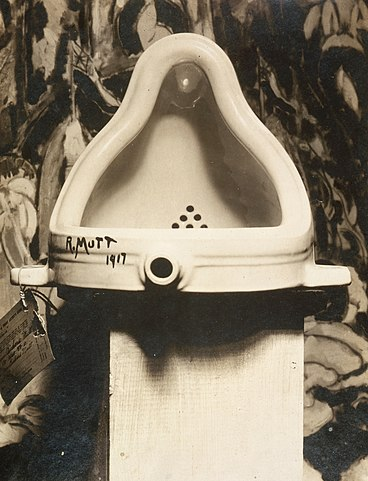
\includegraphics{duchamp}
        \caption{Marcel Duchamp's "Fountain". A urinal that blew peoples minds \url{https://www.tate.org.uk/art/artworks/duchamp-fountain-t07573}.}
        \labfig{duchamp}
\end{marginfigure}

Generative models will come up with amazing (but derivative) works of art, But, they will never "change the game". A model of sculpture trained on past sculptures in 1917 will never come up with Marcel Duchamp's "Fountain". There is a term that machine learning engineers use for this, when the rules of the game are changed, it's called "Concept Drift".

\section{Concept Drift and the End of Usefulness}

Concept drift refers to the phenomenon where the distribution of data changes over time, causing the performance of AI models built on historical data to degrade. The model becomes less useful because it is trained to make predictions based on the relationship between the inputs and outputs in the data it was trained on, and if this relationship changes, the model may start making incorrect predictions. This is particularly problematic in real-world applications, where the data is constantly evolving and the relationship between inputs and outputs is subject to change. To mitigate the effects of concept drift, it is often necessary to continually retrain AI models on updated data.

The frequency with which an AI model needs to be retrained to mitigate the effects of concept drift depends on several factors, including the rate at which the data distribution changes, the size and complexity of the model, and the availability of computational resources.

\begin{marginfigure}[-5.5cm]
        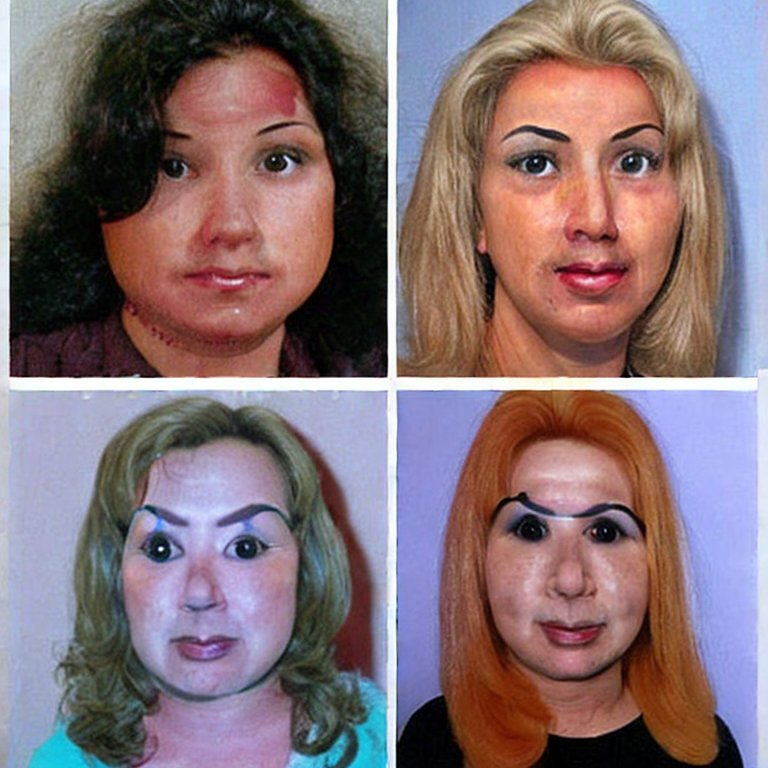
\includegraphics{plastic}
        \caption{"Plastic surgery gone wrong" made with Stable Diffusion. Imagine a model that classifies images as "human face" or "not human face", and imagine that model was trained on images of human faces before 1900, maybe you would not be surprised if you gave it a picture of a human face that had a lot of cosmetic surgery done to it, and that model might say "this is not a human face", the idea of what a human face is has changed over time. This is called "concept drift".}
        \labfig{plastic}
\end{marginfigure}

For some applications with relatively stable data distributions, retraining the model once every few months or even once per year may be sufficient. However, in other applications where the data is changing rapidly, it may be necessary to retrain the model more frequently, such as once per week or even once per day.

Ultimately, the frequency of retraining will depend on the specific requirements of the application, and the trade-off between the cost of retraining and the potential cost of incorrect predictions. In general, it's recommended to monitor the performance of the model over time and to retrain it as needed to ensure that it remains accurate and relevant.

As an example, think about facial recognition models. Facial recogniton models can recognize faces they've seen before, and to have a "perfect" facial recognition model for everyone in the world, you would need to retrain the model on every new face as fast as people were born, or as fast as peoples faces change due to aging or horrific motorcycle accidents. The rate at which you need to retrain the model to maintain it's accuracy depends on how fast new faces are added to the population.\sidenote{This "facial recognition" model is different than the plastic surgery example above, this model is the model that takes a face and says "this is a picture of Brad Pitt" or "this is a picture of Joe Biden" but if you want the model to "recognize" every one in the world, it needs to see everyones face at least once. That is my pedantic but important point I'm making here.}

If a deployed AI model is not monitored, there are several risks that can emerge:

\begin{itemize}
\item Accuracy degradation: As the data distribution changes over time, the model may become less accurate, leading to incorrect predictions. This can result in financial losses, reduced customer satisfaction, or even harm to individuals.
\item Bias amplification: AI models can be biased, and if this bias is not monitored and addressed, it can be amplified over time as the model continues to make incorrect predictions. This can result in discriminatory outcomes, such as unequal treatment of individuals based on protected characteristics such as race, gender, or age.
\item Legal liability: In some cases, incorrect predictions made by AI models can result in legal liability, particularly if the model is being used to make decisions that have significant consequences, such as in the criminal justice system or in medical diagnosis.
\item Reputational damage: If an AI model is making incorrect predictions, it can damage the reputation of the organization deploying the model, potentially leading to a loss of customers or investors.
\end{itemize}

Therefore, it is important to monitor AI models once they are deployed, and to take action to address any issues that arise, such as retraining the model or adjusting its parameters, in order to mitigate these risks and ensure that the model continues to perform well over time.

\section{The Impossibility of Fairness}

Achieving fairness in AI models can be challenging, and to some extent it may be impossible to completely eliminate all forms of bias. This is because AI models are trained on historical data, which may contain biases and disparities that are perpetuated in the model's predictions. One can attempt to "fix the training set"but in practice models will continue to bias their prediction to past data, or their creators careful curation of the past.\sidecite{Christian2020} 

However, it is possible to reduce the impact of bias in AI models through careful design and monitoring of the model's performance. This may include techniques such as fairness constraints, algorithmic transparency, and regular auditing of the model's predictions to identify and address any issues of bias.

It's important to note that fairness is a complex and multi-faceted concept, and different definitions of fairness may be appropriate for different applications. For example, some definitions of fairness may prioritize equal treatment of all individuals, while others may prioritize proportional representation or equal opportunities.

Ultimately, the extent to which fairness is achievable in AI models will depend on the specific requirements of the application and the level of effort that is put into designing and monitoring the model to ensure that it is making fair and unbiased predictions.

\section{Transfer Learning Everywhere}

Transfer learning is a machine learning technique that involves transferring knowledge from one model trained on a task to another model trained on a related task. The idea behind transfer learning is that a model that has been trained on one task can be fine-tuned for another task, reducing the amount of labeled data required to train the new model.

For example, imagine that you have a large convolutional neural network (CNN) that has been trained to recognize objects in natural images. You can use the knowledge learned by this model as a starting point to train a new model that recognizes objects in medical images, such as X-rays or MRI scans. The new model can start with the weights of the pre-trained CNN and fine-tune them on the new task, using a much smaller amount of labeled data than would be required to train the model from scratch.\sidenote{Transfer learning is taking data from a different domain, and pointing the model at a new task where data is hard to come by. Think if you tried to "catch bigfoot" using AI, since you have no data on bigfoot you would maybe use a human face detector and stick in on cameras in the woods to try and find a human-like face out there. It could work wonderfully and you could catch bigfoot, or it could turn out that you made a logical leap and bigfoots face doesn't look anything like a humans, so your use of human data to catch bigfoot was wrong}

Transfer learning can be useful in many different applications, particularly when labeled data is scarce or expensive to obtain. By leveraging knowledge from a pre-trained model, transfer learning can help to improve the performance of new models, reduce the amount of data required for training, and accelerate the development of new machine learning applications.

If the past is not like the future, you are doing transfer learning. Most models steal data from other sources so are doing transfer learning too. This is fine, but do we know that we are doing this? A model that is deployed in a domain experiencing concept drift and continues to make predictions without being retrained can be considered to be doing a harmful form of transfer learning. This is because the model has been trained on a different distribution of data (the past), and is being applied to a new domain with a different distribution (the present and future).

In traditional transfer learning, the goal is to transfer knowledge from one domain to another related domain, where the data distributions are similar enough to enable the model to make accurate predictions. However, in the case of concept drift, the data distributions are changing over time, and the model is becoming less accurate as a result. 

By continuing to make predictions without being retrained, the model is essentially "transferring" its knowledge from a historical data distribution to a new, changed data distribution, which may not be a valid assumption. This can result in incorrect predictions and other negative outcomes, such as harm to individuals or organizations. \sidenote{Think about your life nad if you "transferred" your model of thinking from when you were 12 years old, to "today" when you are 35 years old, that is a bad model to be operating on! That model needs to be updated. We'll explore many examples of where this is and is not a problem in the next chapter"}

\section{Industrial-Scale Plagarism}

Aside from regurgitating the past and predictions from other domains, deep learning models can also enable plagarism on an industrial scale. Early text generation models could be made to write entire sections of \textit{Harry Potter} when fed the opening lines of a chapter. Even as models grow large and more sophisticated, users, researchers and lawyers are still able to "extract the training data"  from large models\sidecite{Carlini2023}, causing headaches for their creators and adding to the work of intellectual property lawyers. 


To avoid this creators of deep learning models have the following tools at their disposal:

\begin{marginfigure}[-5.5cm]
        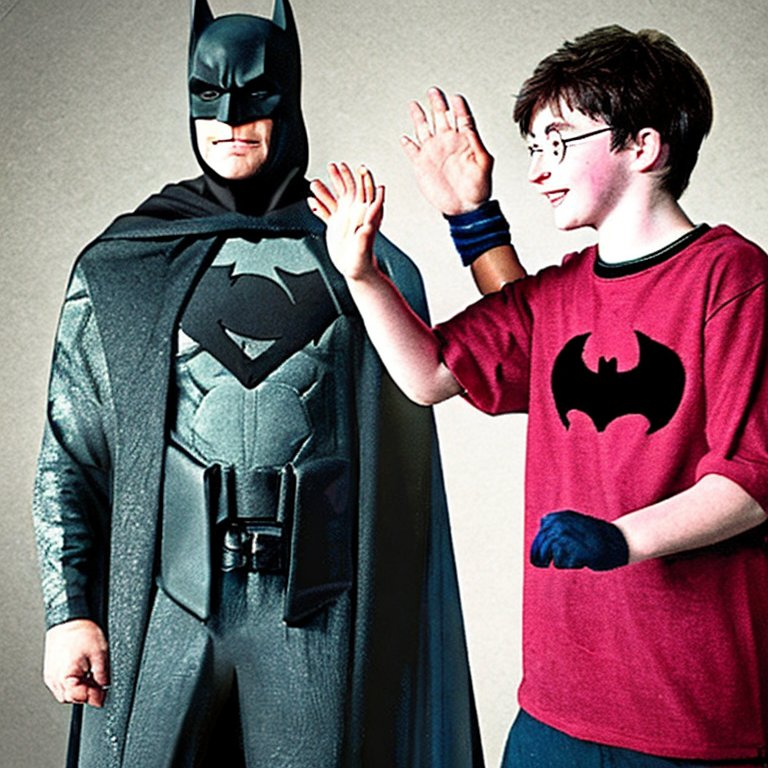
\includegraphics{potter}
        \caption{"Harry Potter and Batman High-fiving" made with Stable Diffusion}
        \labfig{potter}
\end{marginfigure}

\begin{itemize}
\item Best practices in  machine learning: data preprocessing, augmentation, reuglarization, model architeture choices, early stopping and validation are all things that we are taught to do to prevent overfitting.
\item Contractual agreements: Microsoft (owner of github and cocreator of the Github Copilot code generation model) has a special contract for anyone submitting code to github that essentially says that "we are allowed to use this code to train our models, and if our models regenerate your copyrighted code, you can go fuck yourself"
\item Release the kraken: StabilityAI's Stable Diffusion model was released as open source software, they still managed to get sued, but they basically said, "this model was trained on all copyrighted and copylefted images on the web, sometimes it'll generate stuff that violates copyright law, but we are in Germany and will give this thing away for free to the public, and see how the photographers and graphic designers of the world handle it... OKbye!". 
\end{itemize}

These techniques can help to reduce the risk of having AI models reproduce the training data and cause intellectual property disputes, but there is no way to completely eliminate these risks, they are simply side-effects of the method of machine learning that we are doing nowadays.\sidenote{If you are an IP lawyer and need an expert witness, I'm your man \href{mailto:brad@bradflaugher.com}{brad@bradflaugher.com}}

\section{Humans Love Computers}

It turns out the most potent combination is a smart AI paired with a smart person. \sidenote{Funnily enough at Wharton I recently took a class where Dr. Cade Massey said basically "If you want to bring people along and get them to use your model, let them play with the ouput a bit, allowing for even the slightest bit (2\%) adjustment in the outputs will get users to adopt your model much faster}

Once upon a time, Garry Kasparov, a legendary chess player, organized a tournament where humans and AI could compete together. The tournament was designed to showcase the strengths of both humans and AI, and how they could work together to achieve incredible results.

The tournament consisted of several rounds, with each round featuring a human player paired with an AI chess program. The human player would make the first move, and then the AI program would make its move, with the pair working together to win the game.

At the start of the tournament, the human players were skeptical of their AI partners, thinking that the machines would just take over and make all the decisions. But as the tournament progressed, they quickly realized that their AI partners were able to provide valuable insights and help them make better moves.

One team in particular, made up of a seasoned chess player and a cutting-edge AI program, stood out from the rest. The combination of the player's experience and the AI's computational power allowed them to anticipate their opponents' moves and make strategic decisions that no human could have made on their own.

In the final round, the team faced off against the reigning champions, a pair of world-class chess players. The game was intense, with both sides making bold moves and calculating intricate strategies. In the end, the human-AI team emerged victorious, much to the surprise of the crowd.

The tournament was a huge success, and showed that when humans and AI work together, they can achieve amazing things. The tournament participants learned that AI is not just a tool, but a valuable partner, and that by combining their strengths, they could achieve results that neither could have accomplished on their own.

The tournament inspired many people to explore the potential of human-AI collaboration, and showed that by embracing technology, we can create a brighter future for all.

AI is an amazing partner, but we need to think for ourselves too. We can't blindly trust AI, but we can use it to inspire and challenge us.\sidecite{mansharamani2020}

\section{Key Takeaways}

\begin{itemize}
    \item \textbf{Models can puke out their training data} cool!
\end{itemize}

